

\documentclass[letterpaper,10pt]{article}
\bibliographystyle{IEEEtran}
%-----------------------------------------------------------
\usepackage[empty]{fullpage}
\usepackage{color}
\usepackage[bookmarks=true,pdfborder={0 0 0}]{hyperref}
\usepackage{graphicx}
\usepackage{movie15}
\usepackage{times}
\newlength{\outerbordwidth}
\pagestyle{empty}
\raggedbottom
\raggedright
\usepackage[svgnames]{xcolor}
\usepackage{framed}
\usepackage{times}
\usepackage{tocloft}
\usepackage{graphicx}
\usepackage{multirow}
\usepackage[utf8]{inputenc}
\usepackage{tabularx}
\usepackage{boxedminipage}
\usepackage{listings}
\usepackage{minitoc}
\usepackage{graphicx}
\usepackage{enumitem}
\usepackage[utf8]{inputenc}
\usepackage[english]{babel}
\usepackage[document]{ragged2e}
\usepackage{bibentry}
\usepackage{tocvsec2}
\usepackage{etoolbox}


\patchcmd{\thebibliography}{\section*{\refname}}{}{}{}

\graphicspath{ {images/} }
\definecolor{mygrey}{gray}{0.7}
\textheight=8.0in
\raggedbottom
\raggedright
\setlength{\tabcolsep}{0in}

% Adjust margins
\addtolength{\oddsidemargin}{-0.375in}
\addtolength{\evensidemargin}{0.375in}
\addtolength{\textwidth}{0.5in}
\addtolength{\topmargin}{-.375in}
\addtolength{\textheight}{0.75in}

%-----------------------------------------------------------
%Custom commands

\definecolor{lightgray}{gray}{0.8}
\newcolumntype{L}{>{\raggedleft}p{0.14\textwidth}}
\newcolumntype{R}{p{0.8\textwidth}}
\newcommand\VRule{\color{lightgray}\vrule width 0.5pt}

%% publication




\newcommand{\resitem}[1]{\item #1 \vspace{-2pt}}
\newcommand{\resheading}[1]{{\large \colorbox{mygrey}{\begin{minipage}{\textwidth}{\textbf{#1 \vphantom{p\^{E}}}}\end{minipage}}}}
\newcommand{\ressubheading}[4]{
\begin{tabular*}{6.5in}{l@{\extracolsep{\fill}}r}
		\textbf{#1} & #2 \\
		\textit{#3} & \textit{#4} \\
\end{tabular*}\vspace{-6pt}}


\newcommand{\setsignature} {\includegraphics[width=3cm,height=0.8cm]{tran.png}}


%-----------------------------------------------------------
\begin{document}

\textbf{ROBIUL ISLAM }  \\
Room no : 3-309 , Dormitory 3 \\ 
Innopolis University \\ 
Universitetskaya St, 1$\kappa$3, \\
Innopolis, Republic of Tatarstan, 420500 \\
% Room no : 514, Dormitory 9  \\
% National Research University Higher School of Economics  \\
% 5 Tsimlyanskaya Ulitsa, Moscow, Russia  \\
Cell : +7 925 321 3093 \\
Email:\href{mailto:r\_islam@live.com}{r\_islam@live.com} \\
Web page : \url{connect2robiul.github.io}

% \begin{tabular*}{7in}{l@{\extracolsep{\fill}}r}
%   & \multirow{7}{*}{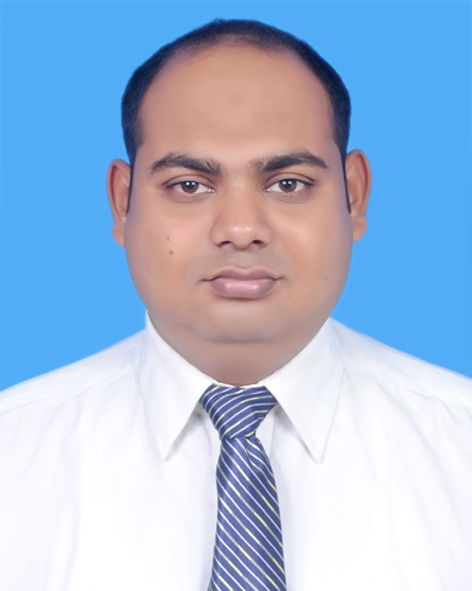
\includegraphics[scale=.65]{rislam.jpg}}
%      \\
% %----nv-------------------------------------------------------
%   \textbf{ROBIUL ISLAM } & \\
% %Room no : 514, Dormitory 9 & \\
% National Research University Higher School of Economics & \\
% 5 Tsimlyanskaya Ulitsa, Moscow, Russia & \\

%   % House No: 49,  Road No :12 & \\
%   % DIT Project, Merul Badda, Dhaka & \\
%   Cell : +7 925 321 3093 &\\
%   Email:\href{mailto:r\_islam@live.com}{r\_islam@live.com} \\
% Web page : \url{connect2robiul.github.io}
%   & 
%   %46/10, DIT Project, Merul Badda  & \\
% %  Dhaka-1212,Bangladesh & \\
% %I.I College Road, Sirajganj Sadar, Sirjganj & \\
%  % Cell : +8801670265300 & \\
%  % Email : r\_islam\@live.com & \\
%  %Email:\href{mailto:r\_islam@live.com}{r\_islam@live.com} & \\
% %LinkedIn : lnkd.in/3GRPSu & \\
% %Hackerrank:https://www.hackerrank.com/connect2robiul & \\
% %freecodecamp : https://www.freecodecamp.com/irobiul & \\
% \end{tabular*}

\vspace{0.1in}

\resheading{Objective}
%\footnotesize
\begin{itemize}
%\item
\resitem{ \justify
% Want to explore my career as a teaching professional in an educational institution that provides handful opportunity of enhancing my analytical ability, creativity and organizing capability so that I can positively contribute to the institutions growth and development through research and introduction of new technology in the field of computer science and technology.
 %Want to explore my career as a software/web professional in an information that provides me a handful opportunity of enhancing my analytical ability,creativity and organizing capability so that I can positively contribute to the institutions growth and development through using new tools in the software developing industry.
 Want to explore my career in such an organization that provides me a handful opportunity of enhancing my analytical ability,creativity and organizing capability so that I can positively contribute to the institutions growth and development.


 }
\end{itemize}

\vspace{0.1in}
\resheading{Experience}
\begin{itemize}
%\item


%\ressubheading{City University}{Dhaka,Bangladesh}{Lecturer of Department of Computer Science and Engineering}{August-2016 to Present}
\item

\ressubheading{Innopolis University}{Innopolis, Russia}{Teaching Assistant}{August-2020 to Present}
\item

\ressubheading{Laboratory for Models and Methods of Computational Pragmatics}{Moscow, Russia}{Research Assistant}{September-2019 to June-2020}

\item

\ressubheading{Intelligent Design \& Dynamic Ltd}{Dhaka,Bangladesh}{Software Engineer}{April-2017 to June-2018}
\item
\ressubheading{Khwaja Yunus Ali University}{Sirajganj,Bangladesh}{Acting Head of Department of Computer Science and Engineering}{April-2016 to August-2016}
\ressubheading{ }{}{Lecturer of Department of Computer Science and Engineering}{Jan-2016 to August-2016 }
%\item
%\ressubheading{Looby Lab}{Dhaka,Bangladesh}{Software Developer}{June-2015 to December-2015}
\item
	\ressubheading{East West University}{Dhaka,Bangladesh}{Graduate Teaching Assistance }{May-2013 to August-2013 }
\ressubheading{}{}{Undergraduate Teaching Assistance}{January-2013 to April-2013}	
\end{itemize}

\resheading{Education}
\begin{itemize}


\item
	\ressubheading{Innopolis University}{Innopolis, Russia}{Doctor of Philosophy, Neuro-science and Cognitive Technology Lab}{Continue}

\item
	\ressubheading{National Research University Higher School of Economics}{Moscow, Russia}{Master’s Programme 'System and Software Engineering'}{Completed in June 2020}
	\begin{itemize}

		\item  CGPA 8.06 on a scale of 10.0

	\end{itemize}


\item
	\ressubheading{Islamic University of Technology}{Gazipur, Bangladesh}{Master of Science in Computer Science and Engineering }{Completed in August 2018}
\begin{itemize}

		\item  CGPA 3.13  on a scale of 4.0

	\end{itemize}
	
\item
	\ressubheading{East West University}{Dhaka,Bangladesh}{Bachelor of Science in Computer Science and Engineering}{Completed in April-2013}
	\begin{itemize}
		\item  CGPA 3.30 on a scale of 4.0

	\end{itemize}


\end{itemize}

\resheading{Project}

\begin{itemize}
\resitem{Nurse Calling system}
\begin{description}
\item
  {\justify \it{This project is built with python flask microframework having or receiving the mqtt real-time call. It helps to collect and sent the signal to Arduino device. }}
\end{description}
\resitem{Vendor Management System}
\begin{description}
\item
  {\justify \it{User management system that helps users for vendor management}}
\end{description}
\resitem{Personal Work}
\begin{description}
\item
  {\justify \it{Successfully uploaded Django software in AWS and Heroku}}
\end{description}
\end{itemize}

\resheading{Research Works}

\begin{itemize}

\resitem{Sequence mining for searching demographic patterns}
\begin{description}
\item
  {\justify \it{This course work is focus on SHAP value(python) to white box. testing. } }Publish: Muratova2019 (Book Chapter)
\end{description}

\resitem{Alphabet strokes recognition in unconstrained Air Writing using Depth Information}
\begin{description}
\item
  {\justify \it{The  thesis work is focusing on video based alphabet strokes recognition of English Capital Letters in air writing by using depth information technology.}} Publish : Islam2016(Short paper)
\end{description}
\resitem{Evolutionary Algorithm for Graph Coloring Problem}
\begin{description}
\item
  {\justify \it{The undergraduate thesis work was focused on the mutation of evolutionary algorithm. Binary encoding has been introduced here for Graph Coloring Problem. Through analysis it has been idealized that introduction of binary encoding has been found facilitating in mutation, evaluation, immune system and merging color easily and also reducing coloring dynamically. }}
\end{description}
\end{itemize}

%\newpage
\resheading{Achievement}
\begin{description}
	\item \textbf{Full Scholarship ,  Innopolis University 2020-24}
\item \textbf{Nomination $<<SILVER \: \: \:  CHILD>>$ Golden HSE Award 2019}
	\item \textbf{Finalist of The Ilya Segalovich Award ,Honor date: Apr 2018, Honor Issuer: Yandex}
	\item \textbf{State Academic Scholarship , National Research University Higher School of Economics 2018-20}
	\item \textbf{IEEE VOLT program Graduate 2017}
\item \textbf{ICT Division Fellowship from ICT Division,Government of the People's Republic of Bangladesh}
\end{description}

\resheading{Publications}
\begin{thebibliography}{}


\bibitem{}
Anna Muratova, \textbf{Robiul Islam}, Ekaterina Mitrofanova, Dmitry I. Ignatov \emph{Searching for Interpretable Demographic Patterns}, in: Proceedings of the Fifth Workshop on Experimental Economics and Machine Learning at the National Research University Higher School of Economics co-located with the Seventh International Conference on Applied Research in Economics (iCare7) Aachen : CEUR Workshop Proceedings, 2019. P. 18-31.

\bibitem{}
Md Rafiqul Islam, Md Abu Raihan Mostafa Kamal, Naznin Sultana, Mohammad Ali Moni, \textbf{Robiul Islam} and Anwaar Ulhaq \emph{Depression Detection Using K-Nearest Neighbors (KNN) Classification Technique}, International Conference on Computer, Communication, Chemical, Materials and Electronic Engineering, 2018 , pages 1-4, 2018  

\bibitem{}
\textbf{Robiul Islam}, Hasan Mahmud, Md. Kamrul Hasan,Husne Ara Rubaiyeat \emph{Alphabet Recognition in Air Writing Using Depth Information}, ACHI 2016 : The Ninth International Conference on Advances in Computer-Human Interactions,page 299-301, April-2016, Venice Italy.ISBN: 978-1-61208-468-8

\end{thebibliography}
\resheading{Workshop/ Online course }
\begin{itemize}

\resitem{\textbf{Workshop on creative questions}, March 19, 2014, Khwaja Yunus Ali University }
\resitem{\textbf{Full Stack Development}, Running ,Free Code Camp}
\resitem{\textbf{IEEE Pro Talks 2015}, 10-Oct-2015 , IEEE Bangladesh Section , BUET }
\resitem{\textbf{C\#/ASP.Net under Hitech Park}, 1-Jan-2015 to 14-May-2015 (144 hours), IBCS - Primax Software
Bangladesh Ltd.}
\resitem{\textbf{Cloud Computing and Big Data - A Paradigm Shift in ICT} ,1 to 5 December 2014, Islamic University of Technology, Dhaka, Bangladesh}
\end{itemize}






\resheading{Skills}

\begin{description}
\item
\resitem{\textbf{Technical Skills}}
\begin{description}
\item[Programming Languages Basic :] PYTHON, C/C++, MATLAB
\item[Script Language Basic :] html, CSS, javascript , jquery , jquery UI, bootstrap
\item[Using Database:] MySQL, SQL, sqlite , postgres 
\item[Web framework:] Flask, Django
%\item[Using Tools :] Microsoft Office, Pspics, Xampp,\LaTeX, Microsoft SQL Server 2008 R2, OpenCV, Microsoft Kinect, Proteus
\end{description}
\item
\resitem{\textbf{Language Proficiency}}
\begin{description}
\item{Bengali (Native)}
%\item{English (Oral and Verbal)}
\item{English (Proficient)}
\end{description}
\end{description}

 \resheading{Membership}
 \begin{itemize}
 \item
 \ressubheading{Institute of Electrical and Electronics Engineers, \(IEEE\)}{Russia Section(Current)}{Member}{Since January-2012}


 \item
 \ressubheading{Bangladesh Computer Society}{Dhaka,Bangladesh }{Associate Member}{October-2015 to Present}
 \item
 \ressubheading{The American Center}{Bangladesh}{Member}{March-2015 to Present }
 \item
 \ressubheading{ The Institution of Engineers, Bangladesh (IEB)}{Bangladesh}{Associate Member}{July-2016 to Present }

 \end{itemize}

\resheading{Voluntary Activities}
\begin{itemize}
	\item{Volunteer of Software Engineering Conference Russia 2018 }
	\item{ExCom Member, IEEE Bangladesh Section Computer Society Chapter 2018 }
	\item {Advisor, IEEE Bangladesh Section Activities Committee 2017}
\item {Educational Activity Coordinator, 2015 committee of IEEE Young Professionals, Bangladesh Section}
    \item{Event Coordinator at IEEE student Branch, East West University from Aug 1, 2012 to Feb 20, 2013 }
    \item {General Member of East West University Science Club from 2009 to 2013}
\end{itemize}



%%\pagebreak
\resheading{References}\\


\vspace{0.1in}

\begin{tabular*} {7in} {l@{\extracolsep{\fill}}l}
\textbf{\large \href{https://www.hse.ru/en/org/persons/222507810}{Sergey Karapetyan}}  & \textbf{Md. Kamrul Hasan, PhD}\\
Manager & Professor\\
Department of Computer Science and Engineering & Department of Computer Science and Engineering \\
National Research University Higher School of Economics & Islamic University of Technology\\
Moscow, Russia &  Board Bazar, Gazipur 1704, Bangladesh\\
E-mail: skarapetyan@hse.ru &  E-mail : hasan@iut-dhaka.edu\\
Phone extension: 23100 & Cellphone: +8801727149224
\end{tabular*}

\vspace{0.1in}

\begin{tabular*} {7in} {l@{\extracolsep{\fill}}l}
\textbf{\large \href{https://www.hse.ru/en/staff/dima}{Dmitry I. Ignatov} }   \\

Laboratory chair,  \\
Laboratory for Models and Methods of Computational Pragmatics \\
Associate Professor \\
Faculty of Computer Science \\
School of Data Analysis and Artificial Intelligence \\
National Research University Higher School of Economics \\
Moscow, Russia \\ 
Phone: +7(495) 772-9590 Phone extension: 22930 \\
Email : dignatov@hse.ru \\
\end{tabular*}



% \resheading{Certification}
% \vspace{0.2in}
% I, hereby the undersigned, confirming that the information given above are true and best of my knowledge.\\
% \vspace{.4in}
% \textbf  {Robiul Islam}

%%
% \closing{Yours faithfully,\\
% \fromsig{\includegraphics[scale=1]{sign.jpg}} \\
% \fromname{Your name}
%%

\end{document} 
